\subsubsection{General problem description}
In this example, we solve a optimization problems from 
fluid dynamics. The configuration is similar to 
the fluid optimization problem proposed by Roland Becker 
``Mesh adaption for stationary flow control'' (2000).

The configuration
    comes from the original fluid benchmark problem
    and has been modified to reduce drag around the
    cylinder. To gain the solvability of
    the optimization problem we add a quadratic
    regularization term to the cost functional.


\begin{figure}[h]
\centering
    {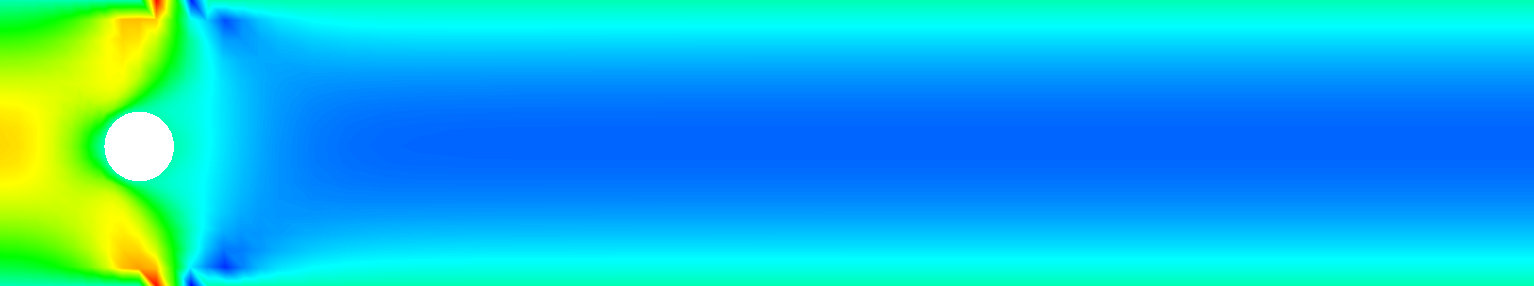
\includegraphics[width=7cm]{Documentation/visit_Nov_15_2013_0000_a.png}}
    {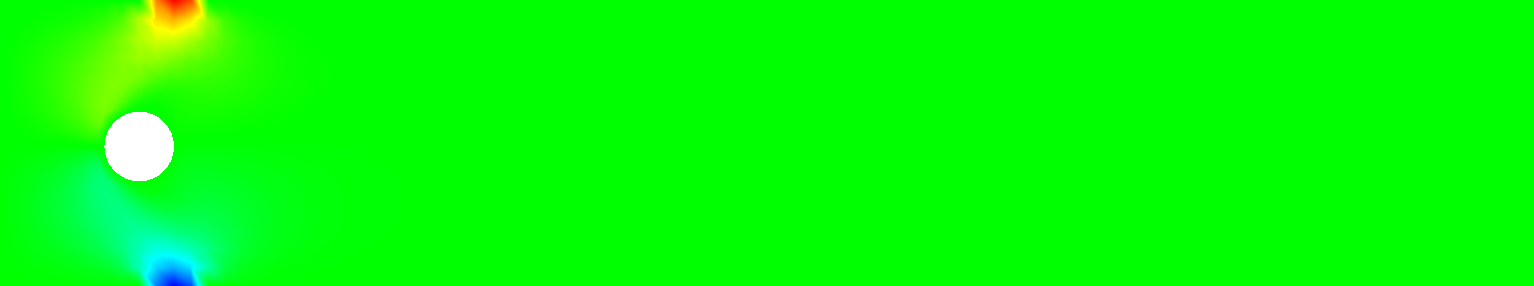
\includegraphics[width=7cm]{Documentation/visit_Nov_15_2013_0001_a.png}}
  \caption{Configuration of the cylinder-drag minimization problem. 
By sucking out the fluid (right the $y$-velocity), 
the force on the cylinder is reduced. At left, the $x$-velocity field 
is shown. Behind the cylinder, almost no fluid goes from left to right, 
which is shown in blue color.}
\end{figure}

The computational domain is denoted by $\Omega$ with the 
boundary $\partial\Omega
= \Gamma_in \cup \Gamma_out \cup \Gamma_Q \cup \Gamma_w$, 
where $\Gamma_in$ and $\Gamma_out$ denote the inflow and outflow
boundaries, respectively. On $\Gamma_in$, we prescribe a fixed parabolic 
inflow profile. The part(s) $\Gamma_w$ denote the top and bottom 
boundaries. Finally, $\Gamma_Q$, represent Neumann control boundaries. Here,
we prescribe 
\[
\rho\nu \partial_n v - pn = qn \quad\text{on } \Gamma_Q
\] 
where $n$ denotes the outer unit normal to $\Gamma_Q$. 

The state equations are given by: Find $v$ and $p$ such that
\begin{align*}
- \nabla\cdot \sigma(v,p) + v\cdot \nabla v = 0,\\
\nabla\cdot v = 0
\end{align*}
with $\sigma(v,p) = -pI + \rho\nu(\nabla v + \nabla v^T)$.

\begin{remark} Since, we use the 
symmetric stress tensor, we need to subtract the nonsymmetric part 
on the outflow boundary, related to the do-nothing condition.
$\diamond$
\end{remark}

The control $q$ enters via the weak formulation. It reads,
\begin{align*}
a(q,v,p)(\phi) = (\sigma(v,p), \phi) + (v\cdot \nabla v, \phi) 
+ \langle q, \phi\cdot n \rangle + (\nabla\cdot v, \chi) = 0,
\end{align*}




The target functional is considered as 
\[
k(v,p) = \int_{\Gamma_O} n\cdot \sigma(v,p)\cdot d \, \mathrm{d}s,
\]
where $\Gamma_O$ denotes the cylinder boundary, and $d$ is a vector in the
direction
of the mean flow. For theoretical and numerical reasons, this functional 
needs to be regularized, including the control variable $q$, such that
\[
K(q,v,p) = k(v,p) + \frac{\alpha}{2}||q - q_0||^2,
\] 
where $\alpha$ is the Tikhonov parameter and $q_0$ some 
reference control. 

The rest of the program is similar to the previous optimization problems where
we formulate the state equation in a weak form $a(v,p)(\phi)$ such that the 
final problem reads
\[
K(q,v,p) \rightarrow \text{min} \quad \text{s.t.} \quad a(q,v,p)(\phi) = 0.
\]


\subsubsection{Program description}
The implementation of this example does not introduce any new \dope{}-specific
features but shows that more complicated equations such as the Navier-Stokes 
system can be used as forward problem for the optimization process. 
This example builds on the previous Example \ref{OPT_Stat_Param_Lin_Ellipt}.

